%input macros (i.e. write your own macros file called MacroFile1.tex)
%% Personal macros
\newcommand{\JENC}{Jens Enzo Nyby Christensen}
\newcommand{\email}{jens@jensenzo.com}

%% Editing macros
\newcommand{\todo}[1]{\textcolor{red}{@TODO: #1}}

%% Maths macros
\newcommand{\argmin}[1]{\underset{#1}{\mathrm{argmin}}}
\newcommand{\argmax}[1]{\underset{#1}{\mathrm{argmax}}}

%% Functional short-hands and inserts
\newcommand{\PdfPsText}[2]{
  \ifpdf
     #1
  \else
     #2
  \fi
}

\newcommand{\IncludeGraphicsH}[3]{
  \PdfPsText{\includegraphics[height=#2]{#1}}{\includegraphics[bb = #3, height=#2]{#1}}
}

\newcommand{\IncludeGraphicsW}[3]{
  \PdfPsText{\includegraphics[width=#2]{#1}}{\includegraphics[bb = #3, width=#2]{#1}}
}

\newcommand{\InsertFig}[3]{
  \begin{figure}[!htbp]
    \begin{center}
      \leavevmode
      #1
      \caption{#2}
      \label{#3}
    \end{center}
  \end{figure}
}



%%% Local Variables:
%%% mode: latex
%%% TeX-master: "~/Documents/LaTeX/CUEDThesisPSnPDF/thesis"
%%% End:


\documentclass[oneside,12pt]{Classes/CUEDthesisPSnPDF}
\usepackage{color}

\ifpdf
    \pdfinfo { /Title  (Thesis title)
               /Creator (TeX)
               /Producer (pdfTeX)
               /Author (\JENC \email)
               /CreationDate (D:20120606150614)  %format D:YYYYMMDDhhmmss
               /ModDate (D:20030815213532)
               /Subject (Writing a PhD thesis in LaTeX)
               /Keywords (PhD, Thesis)}
    \pdfcatalog { /PageMode (/UseOutlines)
                  /OpenAction (fitbh)  }
\fi

\title{PhD Thesis title which will be fairly long I suspect}

\ifpdf
  \author{\href{mailto:\email}{\JENC}}
  \collegeordept{\href{http://www.eng.cam.ac.uk}{Department of Engineering}}
  \university{\href{http://www.cam.ac.uk}{University of Cambridge}}
% insert below the file name that contains the crest in-place of 'UnivShield'
  \crest{
\includegraphics[width=30mm]{UnivShield}}
\else
  \author{\JENS}
  \collegeordept{Department of Engineering}
  \university{University of Cambridge}
% insert below the file name that contains the crest in-place of 'UnivShield'
  \crest{
\includegraphics[bb = 0 0 292 336, width=30mm]{UnivShield}}
\fi
%
% insert below the file name that contains the crest in-place of 'UnivShield'
% \crest{\IncludeGraphicsW{UnivShield}{40mm}{14 14 73 81}}
%
%\renewcommand{\submittedtext}{change the default text here if needed}
\degree{Doctor of Philosophy}
\degreedate{Degree date yet to be decided}

% turn of those nasty overfull and underfull hboxes
\hbadness=10000
\hfuzz=50pt

% Put all the style files you want in the directory StyleFiles and usepackage like this:
\usepackage{StyleFiles/watermark}


\begin{document}

%\language{english}

 \renewcommand\baselinestretch{1.2}
\baselineskip=18pt plus1pt

% A page with the abstract on including title and author etc may be
% required to be handed in separately. If this is not so, then comment
% the below 3 lines (between '\begin{abstractseparte}' and
% 'end{abstractseparate}'), normally like a declaration ... needs some more
% work, mind as environment abstracts creates a new page!
% \begin{abstractseparate}
%   
% Thesis Abstract -----------------------------------------------------


%\begin{abstractslong}    %uncommenting this line, gives a different abstract heading
%\begin{abstracts}        %this creates the heading for the abstract page
\begin{thesissummary}
Impact related audio pulses are a frequent, and mostly undesirable, occurrence on many modern integrated devices. This thesis has explored two aspects of these pulses in real-time audio streams. Firstly a functional view of pulses that aimed to localise impact sites of touch events solely based on a single audio stream. This work is framed as a proposed touchscreen interface. Secondly, the pulses were considered noise and a real-time single-channel detection and restoration system was constructed for a telecommunication application.

Results showed that it is possible, using a large aligned ensemble of training pulses and PCA factorisation, to accurately and robustly estimate the origin of impact sites on a device. It was also found that the use of PCA enabled acceptance of a higher degree of variability within individual spots. Results also showed that pulses could successfully be modelled as linear scalings of a combination of components, yielding increased performance. A generalised multi-channel implementation further increased performance of the system. It was also found that the wavelet basis is accurately able to detect transient noise pulses with high temporal accuracy. False detection rates were compared with competing methods on a large corpus of data and the proposed model perform similarly or better. Furthermore it was found that real-time interpolation of missing data was possible directly on the wavelet coefficients. These results were verified with both objective perceptual models, standard error metrics and subjective listening tests.



\end{thesissummary}
%\end{abstracts}
%\end{abstractslong}


% ----------------------------------------------------------------------


%%% Local Variables:
%%% mode: latex
%%% TeX-master: "../thesis"
%%% End:

% \end{abstractseparate}




% Using the watermark package which is in StyleFiles/
% and to remove DRAFT COPY ONLY appearing on the top of all pages comment out below line
%\watermark{DRAFT COPY ONLY}


\maketitle

%set the number of sectioning levels that get number and appear in the contents
\setcounter{secnumdepth}{3}
\setcounter{tocdepth}{3}

\frontmatter
% Thesis Dedictation ---------------------------------------------------

\begin{dedication} %this creates the heading for the dedication page

I would like to dedicate this thesis to my loving parents ...

\end{dedication}

% ----------------------------------------------------------------------

%%% Local Variables: 
%%% mode: latex
%%% TeX-master: "../thesis"
%%% End: 

% Thesis Acknowledgements ------------------------------------------------


%\begin{acknowledgementslong} %uncommenting this line, gives a different acknowledgements heading
\begin{acknowledgements}      %this creates the heading for the acknowlegments


And I would like to acknowledge ...


\end{acknowledgements}
%\end{acknowledgmentslong}

% ------------------------------------------------------------------------

%%% Local Variables: 
%%% mode: latex
%%% TeX-master: "../thesis"
%%% End: 


% Thesis Abstract -----------------------------------------------------


%\begin{abstractslong}    %uncommenting this line, gives a different abstract heading
%\begin{abstracts}        %this creates the heading for the abstract page
\begin{thesissummary}
Impact related audio pulses are a frequent, and mostly undesirable, occurrence on many modern integrated devices. This thesis has explored two aspects of these pulses in real-time audio streams. Firstly a functional view of pulses that aimed to localise impact sites of touch events solely based on a single audio stream. This work is framed as a proposed touchscreen interface. Secondly, the pulses were considered noise and a real-time single-channel detection and restoration system was constructed for a telecommunication application.

Results showed that it is possible, using a large aligned ensemble of training pulses and PCA factorisation, to accurately and robustly estimate the origin of impact sites on a device. It was also found that the use of PCA enabled acceptance of a higher degree of variability within individual spots. Results also showed that pulses could successfully be modelled as linear scalings of a combination of components, yielding increased performance. A generalised multi-channel implementation further increased performance of the system. It was also found that the wavelet basis is accurately able to detect transient noise pulses with high temporal accuracy. False detection rates were compared with competing methods on a large corpus of data and the proposed model perform similarly or better. Furthermore it was found that real-time interpolation of missing data was possible directly on the wavelet coefficients. These results were verified with both objective perceptual models, standard error metrics and subjective listening tests.



\end{thesissummary}
%\end{abstracts}
%\end{abstractslong}


% ----------------------------------------------------------------------


%%% Local Variables:
%%% mode: latex
%%% TeX-master: "../thesis"
%%% End:


\tableofcontents
\listoffigures
\printnomenclature  %% Print the nomenclature
\addcontentsline{toc}{chapter}{Nomenclature}


\mainmatter

%%% Thesis Introduction --------------------------------------------------
\chapter{Introduction}\label{ch:Introduction}
\ifpdf
    \graphicspath{{Introduction/IntroductionFigs/PNG/}{Introduction/IntroductionFigs/PDF/}{Introduction/IntroductionFigs/}}
\else
    \graphicspath{{Introduction/IntroductionFigs/EPS/}{Introduction/IntroductionFigs/}}
\fi

\section{Problem overview}
Transient pulses in an audio stream originating from the physical interaction with a device, are a common feature of modern integrated devices. Microphones are typically incorporated into laptop computers, mobile phones and tablets due to their low price and relatively high utility in relation to single or multi-channel audio recordings or for noise or echo-cancellation applications. The primary function of the embedded microphones is typically to pick up external sounds (external to the device), but as a consequence of the mechanical construction microphones tend to pick up physical interactions with the device as well. In devices with embedded keyboards typing will often produce clearly audible transient pulses in the audio stream, e.g. a conference call, which may be considered a nuisance and even cause a loss of intelligibility. Even interactions via non-physical keys, e.g. touchscreens, will produce a clearly audio pulse in the audio stream of a device. While these audible pulses would be considered a nuisance in the context of a conference call, it is possible that they could provide additional information about the origin of touch interactions in others.

\section{Aims and objectives}
The work presented here will consider two aspects of impact related audio pulses. Firstly the pulses will be considered from a functional perspective as a means for localising impacts, and secondly the pulses will be considered as an annoyance or deleterious effect in the form of noise. It is noted that these two perspectives are not necessarily mutually exclusive, i.e. one might wish to both classify and then remove such a transient.

\subsection{Acoustic pulse recognition (APR)}
\emph{Is it possible to accurately infer the origin of a device-interaction solely based on the audible pulse generated from the interaction?}
This question will be considered primarily from the perspective of a single-channel input and will focus on methods that are computationally realisable in a real-time scenario. The problem will be framed as a touchscreen implementation and will be referred to as acoustic pulse recognition (APR). The performance of the methods developed will be compared and contrasted and various practical concerns associated with the particular application will be discussed. An extension of the application will seek to generalise the application to multiple channels.

An example of a pulse associated with the interaction with a device is shown in Figure~\ref{fig:singleSampleTap.png}. This pulses is recorded from a standard mobile phone (more details in section~\ref{sec:APRsystem}), and the majority of the pulses has decayed after approximately 7 ms.

\begin{figure}
  \begin{center}
    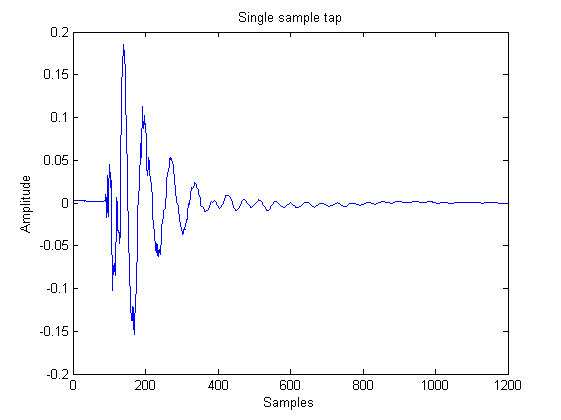
\includegraphics[width=110mm]{singleSampleTap.png}
    \caption{A sample pulse from a mobile phone. Sampled at 44.1 kHz.}\label{fig:singleSampleTap.png}
  \end{center}
\end{figure}

A successful application of a classification algorithm relies on the similarity of pulses from identical impact sites and dissimilarity from those from other sites. Figure~\ref{fig:twotwoSampleTap.png} shows an example of four pulses: two from one spot (blue) and two from a different spot (red). It is clearly seen in Figure~\ref{fig:twotwoSampleTap.png} that while the blue pulses are nearly identical their waveforms are vastly different to that of the red pulses. This observation is, as noted, integral to a successful classification algorithm based on this data. In this example all pulse-onsets have been aligned to the same point.

\begin{figure}
  \begin{center}
    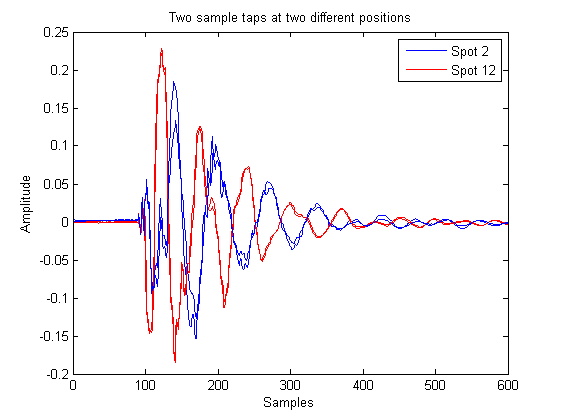
\includegraphics[width=110mm]{twotwoSampleTap.png}
    \caption{Two sets of two sample pulses recorded a two different spots on the mobile phone. Sampled at 44.1 kHz.}\label{fig:twotwoSampleTap.png}
  \end{center}
\end{figure}

While Figure~\ref{fig:twotwoSampleTap.png} shows data obtained in an ideal scenario, pulses will vary greatly depending on factors such as temperature, how the device is suspended and with what it is impacted. The work undertaken in chapters~\ref{ch:APR} and~\ref{ch:MultichannelAPR} will seek to apply this classification algorithm as a real world touch surface application.

% Summary of literature
%A range of applications have been proposed that utilise multiple microphones to implement a touchscreen interface\cite{US8174547}\cite{US8233353}\cite{TouchSystems2006}\cite{US7411581}\cite{WO2006108443}. The functional elements of these methods all rely on their being multiple sources and so the single-channel implementation of the APR system is radically different and should therefore be considered a significant contribution. Not only does the single-channel implementation of the APR system allow for lower hardware cost for integration, it also enables post-hoc integration in system without multiple accessible microphones which currently still is the majority of devices. Work presented in chapter~\ref{ch:APR} is also presented in \cite{Christensen2011} and \cite{US20110316784}.

\subsection{Keyboard stroke removal}
\emph{Is it possible to remove or reduce the effect of transient noise pulses, in particular keyboard stroke noise, on a real-time single channel audio stream for teleconferencing applications?}
This question will again be considered in the context of a realistic teleconferencing scenario. The implementation will be limited by the practical constraints of the webRTC platform and feature a sampling frequency of 16 kHz and buffers of 256 samples with 96 samples of overlap between buffers, leaving 10 ms of new data per buffer. In addition the system needs to be applicable in a real-time scenario setting limits to the computational requirements of the system. The system should be unsupervised, require no training, work on, and remove, a multitude of noise pulses while letting speech signals through unaffected. The system being developed can roughly be divided into two separate parts: a detection stage and a restoration stage. It is the aim to detect pulses reliably while embedded in speech segments, accurately in time and with as few false detections as possible. Restorations of the detected pulses should aim to decrease the nuisance associated with the noise pulses and restored and interpolated segments should be unobtrusive and preferably unnoticeable.

The primary focus of this noise removal algorithm are the noise pulses associated with keyboard typing strokes. As with the more general pulses associated with the classification application the keyboard stroke pulses vary greatly with a range of factors but more importantly they vary between devices. This is a particular issue given that the algorithm specifications requires the algorithm to be unsupervised and will therefore not able to learn the particular signature of keystrokes on a particular device.

Figure~\ref{fig:KeyboardStrokeSlowIntro.pdf} shows an example of the waveform from a single slowly typed keystroke. This single keyboard stroke is noticeably comprised of two individual pulses, where the initial sharply rising pulse is associated with the physical action of the mechanical key being pressed and the secondary lower amplitude pulse nearly 200 ms after the initial pulse is associated with the lifting of the finger from the button. This delay between the two pulses is what defines this keyboard stroke as \emph{slow}, whereas faster typing can leave gaps much shorter. It is also noted that there is a significant slowly decaying low frequency component associated with each individual pulse.

\begin{figure}
  \begin{center}
    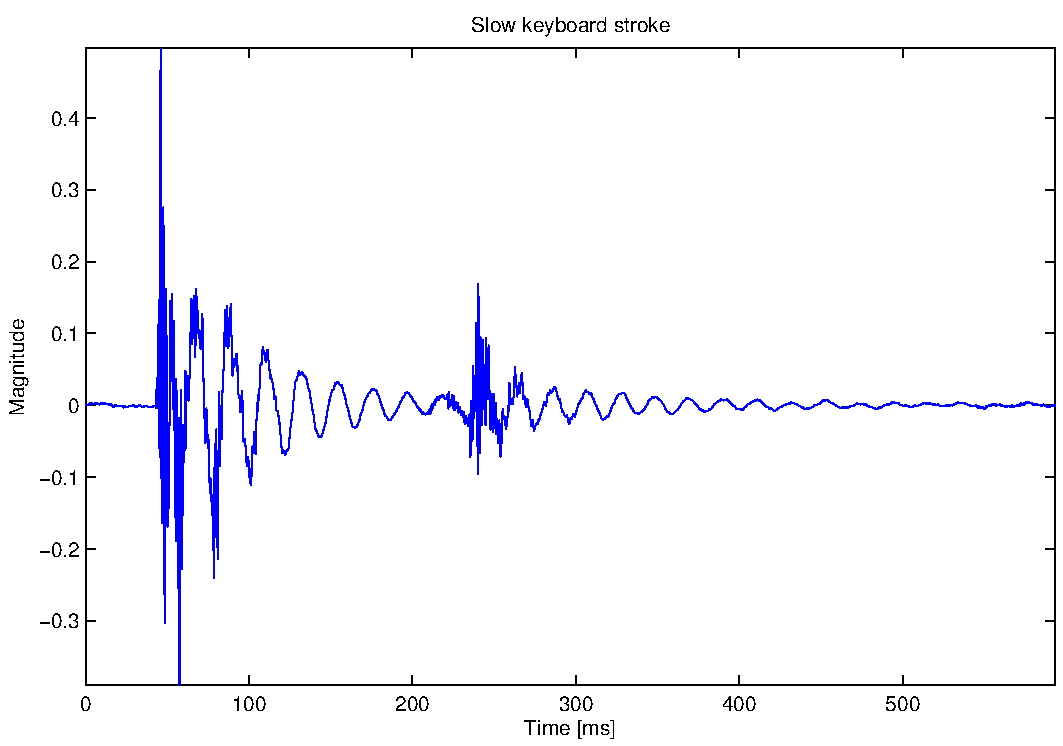
\includegraphics[width=110mm]{KeyboardStrokeSlowIntro.pdf}
    \caption{A sample keystroke sampled at 44.1 kHz.}\label{fig:KeyboardStrokeSlowIntro.pdf}
  \end{center}
\end{figure}

Figure~\ref{fig:shortFastSeq.png} shows the keyboard strokes in the context of a short rapidly typed 5 stroke sequence. The lift-pulses can be seen to appear right before (approximately 10 ms) the second, third and fourth stroke whereas the rest if the lift-pulses are more delayed. It is also noted that while these four primary keystroke-pulses are part of the same sequence they are visually dissimilar. It is also noted that the first stroke clearly shows two distinct pulses in the waveform while an audible evaluation only reveals a single pulse. It is clear that pulses arising from real life typing is extremely varied with only few common features one of which is an initial clear sudden rise noted in the signal amplitude.

\begin{figure}
  \begin{center}
    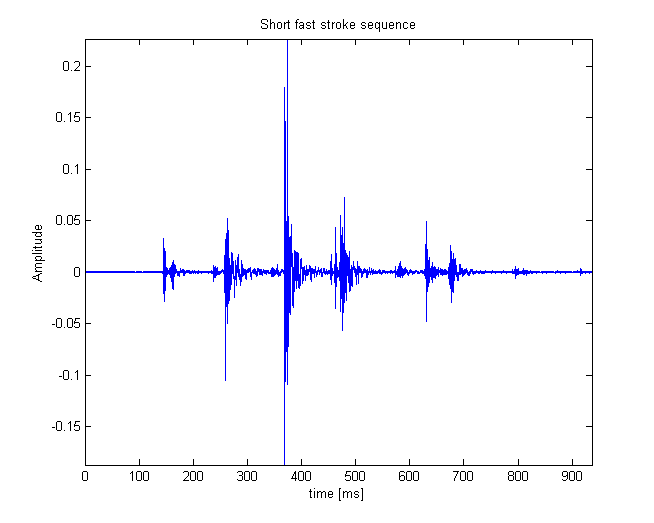
\includegraphics[width=110mm]{shortFastSeq.png}
    \caption{A quickly typed sequence of 5 keyboard strokes sampled at 44.1 kHz.}\label{fig:shortFastSeq.png}
  \end{center}
\end{figure}

Figure~\ref{fig:shortFastSeqSpec.png} shows a spectrogram of the typing sequence displayed in Figure~\ref{fig:shortFastSeq.png}. It is noted that all pulses exhibit a short sudden burst of energy across the spectrum. Even the lift-pulses exhibit this characteristic at a lower level. With each pulses is also a clearly identifiable burst of low frequency energy, in the range of human speech, which clearly outlasts the higher frequency components in time.

\begin{figure}
  \begin{center}
    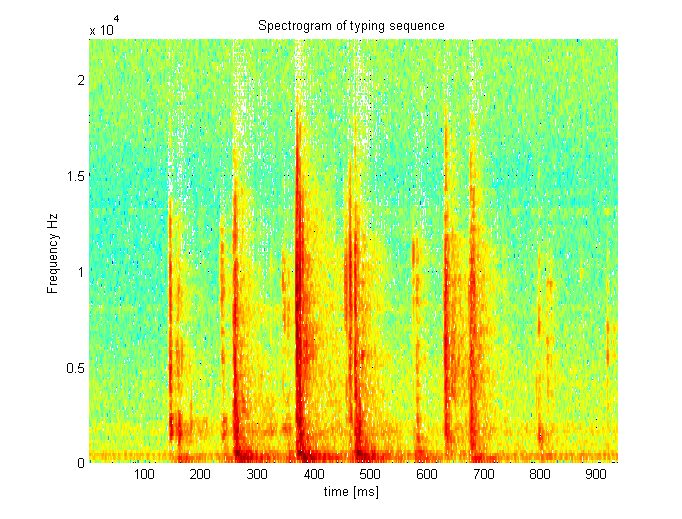
\includegraphics[width=110mm]{shortFastSeqSpec.png}
    \caption{Spectrogram of the same sequence of 5 keystrokes as in Figure~\ref{fig:shortFastSeq.png}. Sampled at 44.1 kHz.}\label{fig:shortFastSeqSpec.png}
  \end{center}
\end{figure}

A thorough investigation of the data associated with this application will be conducted in section~\ref{sec:WPdata}, but with this initial investigation the distinguishing features of interest in keyboard typing pulses are a wide spectral response and rapid onset with lingering low frequency components. The temporal extent of the initial pulses typically range from 30 ms to over 300 ms.

%in the literature (summary)
%A couple of articles have suggested similar systems\cite{Subramanya2007}\cite{Sugiyama2007}\cite{Abramson2007}. \cite{Subramanya2007} and \cite{Sugiyama2007} propose algorithms specifically for the keyboard stroke detection and removal application. All of these methods rely on STFT as a basis for detection using features such as the shape of and change of the power spectrum\cite{Sugiyama2007}, AR estimation error\cite{Subramanya2007}\cite{Kauppinen2002} or a Bayesian speech estimator\cite{Abramson2007}. In \cite{Godsill1998book} various AR based detection methods are proposed and it was found that pairing the AR model with a basis, e.g. a sinusoid, gives a generally applicable approach with improved performance. In \cite{Vaseghi1990} the authors find that AR processes are ``adequate for modelling of speech signals whereas they can not model impulsive disturbances.''.
%
%Restoration approaches applicable to longer gaps ranged from heuristic waveform substitution methods\cite{Goodman1986}\cite{Niediwiecki2001}, pitch based methods modeling speech as spectral peak tracks\cite{Maher1994}\cite{McAulay1986} to AR interpolators\cite{Esquef2006} based on a least squares adaption of the AR process\cite{Godsill1998book}.
%synthesis filters designed to excite the AR model to achieve longer gap extrapolation with lower model orders\cite{Esquef2006}

%\section{Scope of the thesis and contributions to knowledge}

\section{Terminology}
%pulse/impulse
%noise
%Transient noise used when focus on noise.
Throughout the literature the terms \emph{pulse}\cite{Esquef2002a}\cite{Esquef2003a} and \emph{impulse}\cite{Czyzewski1995}\cite{Kauppinen2002a}\cite{Chen2000} have been used interchangeably to refer to a short burst of sound. Generally the use of the term \emph{click}\cite{Czyzewski1995}\cite{Esquef2002}\cite{Godsill1998book} has been associated with physical defects in a recording medium or other extremely short term corruptions. Henceforth the term \emph{pulse} will be used to describe the specific audio signals of interest throughout this work, for its alignment with the already established term acoustic pulse recognition (APR)\cite{TouchSystems2006}. The term \emph{noise}, or the more specific \emph{impulsive noise} and \emph{transient noise}, will only be used to refer to specifically unwanted aspects of the signal and will as such mainly be used in chapters~\ref{ch:TransientNoiseDetection} and \ref{ch:TransientNoiseRestoration}.

%Keyboard stroke pulse (sometimes pulse sequence) vs. single pulse
In chapters~\ref{ch:TransientNoiseDetection} and \ref{ch:TransientNoiseRestoration} the term \emph{keyboard stroke} or \emph{key stroke} will be used to specifically refer to the sequence of disturbances that arise from typing action on a keyboard. These sequences will in many cases encompass a series of \emph{pulses}.

%Chapter~\ref{ch:TransientNoiseRestoration} is commonly referred to as the \emph{restoration} chapter, but the term \emph{reconstruction} has also in some places been applied somewhat interchangeably. In general the term \emph{restore} has been used more generally as any action that aims to alleviate \emph{defects}, \emph{artifacts} or \emph{noise}. \emph{Reconstruct} refers more specifically to situations where samples are discarded and replaced with new estimates. An example of a \emph{restoration} that would not be a \emph{reconstruction} is a scaling action of corrupted samples. In the same chapter the terms \emph{interpolation} and \emph{extrapolation} has been used in some contexts interchangeably. In general \emph{interpolate} is used to refer to action where samples are inserted in between other samples by some means, e.g. linear interpolation, where \emph{extrapolate} refers to the extension of a signal with no pre-defined end points, e.g. prediction. Typically \emph{interpolation} is here more often used to refer to the non-real-time applications that in most cases end up being \emph{extrapolation} when applied in real-time due to the general rule of causality.

\section{Contributions of this thesis}
Work presented in chapter~\ref{ch:APR} is also presented in \cite{Christensen2011} and \cite{US20110316784}.

\section{About this thesis}
This thesis is structured as follows; Following this introductory chapter the literature review is presented in chapter~\ref{ch:LiteratureReview}. Here the surveyed literature is presented in sections relevant to their occurrence in the thesis. Chapter~\ref{ch:APR} introduces the pulse classification or APR system and the main theory. Results are also presented outlining detection performance and the model's sensitivity to certain parameters. Chapter~\ref{ch:MultichannelAPR} presents a multi-channel generalisation of the basic model derived in chapter~\ref{ch:APR}. Results are presented, in Chapter~\ref{ch:MultichannelAPR}, from extensive testing in clean and noisy environments. Chapters~\ref{ch:TransientNoiseDetection} and~\ref{ch:TransientNoiseRestoration} should be considered together as the transient noise suppression system, where chapter~\ref{ch:TransientNoiseDetection} presents methods for the detection of pulses including a proposed pre-processing stage and chapter~\ref{ch:TransientNoiseRestoration} builds on the previous work and considers a number of restoration approaches for the detected pulses. The thesis ends with the conclusions in chapter~\ref{ch:Conclusions}. Here the aims for the work presented in the introduction are reevaluated in the context of the work undertaken. The major contributions are restated and a summary of the proposed future work is presented.

%%% ----------------------------------------------------------------------


%%% Local Variables:
%%% mode: latex
%%% TeX-master: "../thesis"
%%% End:

\chapter{Detection of transients}
% Amplitude detection
% Median-filter detection
% Correlation detection
% Noise burst model (with Wavelets and STFT) (like UKD)
% % Noise burst model w. AR background noise
% Switched noise burst model
% % HMM interpretation


% This is classification?
% Bayesian template based detection
% % Mean template
% % % ML
% % % MAP
% % Multiple components


\ifpdf
    \graphicspath{{Chapter1/Chapter1Figs/PNG/}{Chapter1/Chapter1Figs/PDF/}{Chapter1/Chapter1Figs/}}
\else
    \graphicspath{{Chapter1/Chapter1Figs/EPS/}{Chapter1/Chapter1Figs/}}
\fi

\section{First Paragraph}
And now I begin my first chapter here, which is nice: F $F(x) = y x^2$ ...

Here is an equation\footnote{the notation is explained in the nomenclature section :-)}:
\begin{eqnarray}
CIF: \hspace*{5mm}F_0^j(a) &=& \frac{1}{2\pi \iota} \oint_{\gamma} \frac{F_0^j(z)}{z - a} dz
\end{eqnarray}
\nomenclature[zcif]{$CIF$}{Cauchy's Integral Formula}                                % first letter Z is for Acronyms
\nomenclature[aF]{$F$}{complex function}                                                   % first letter A is for Roman symbols
\nomenclature[gp]{$\pi$}{ $\simeq 3.14\ldots$}                                             % first letter G is for Greek Symbols
\nomenclature[gi]{$\iota$}{unit imaginary number $\sqrt{-1}$}                      % first letter G is for Greek Symbols
\nomenclature[gg]{$\gamma$}{a simply closed curve on a complex plane}  % first letter G is for Greek Symbols
\nomenclature[xi]{$\oint_\gamma$}{integration around a curve $\gamma$} % first letter X is for Other Symbols
\nomenclature[rj]{$j$}{superscript index}                                                       % first letter R is for superscripts
\nomenclature[s0]{$0$}{subscript index}                                                        % first letter S is for subscripts

\section{Second Paragraph}
and here I write more ...

\subsection{sub first paragraph}
... and some more ...

Now I would like to cite the following: \cite{latex} and \cite{texbook}
and \cite{Rud73}.

I would also like to include a picture ...

\begin{figure}[!htbp]
  \begin{center}
    \leavevmode
    \ifpdf
      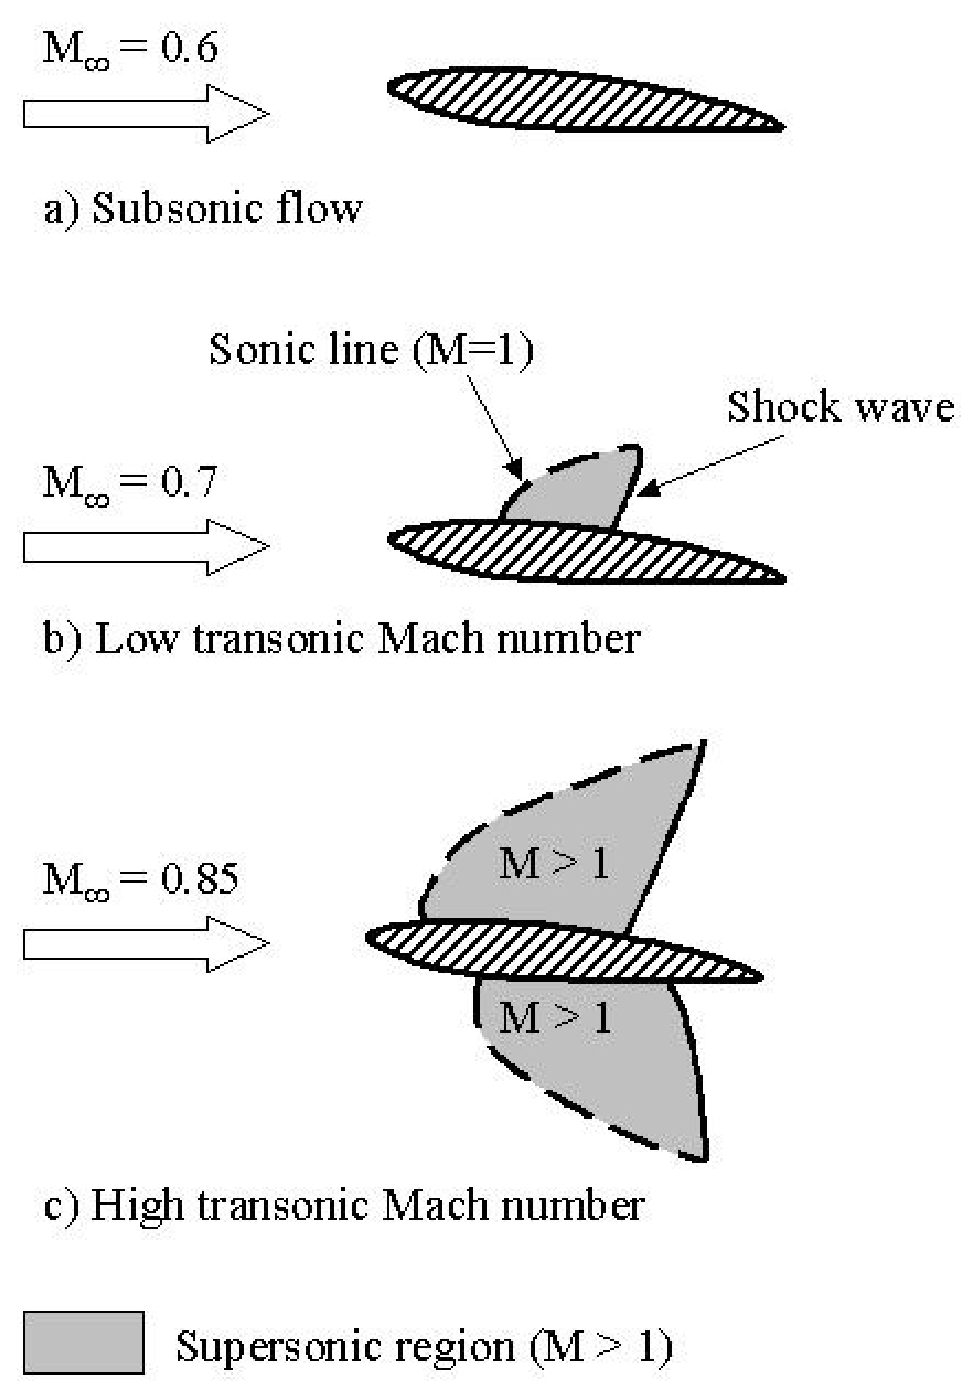
\includegraphics[height=6in]{aflow}
    \else
      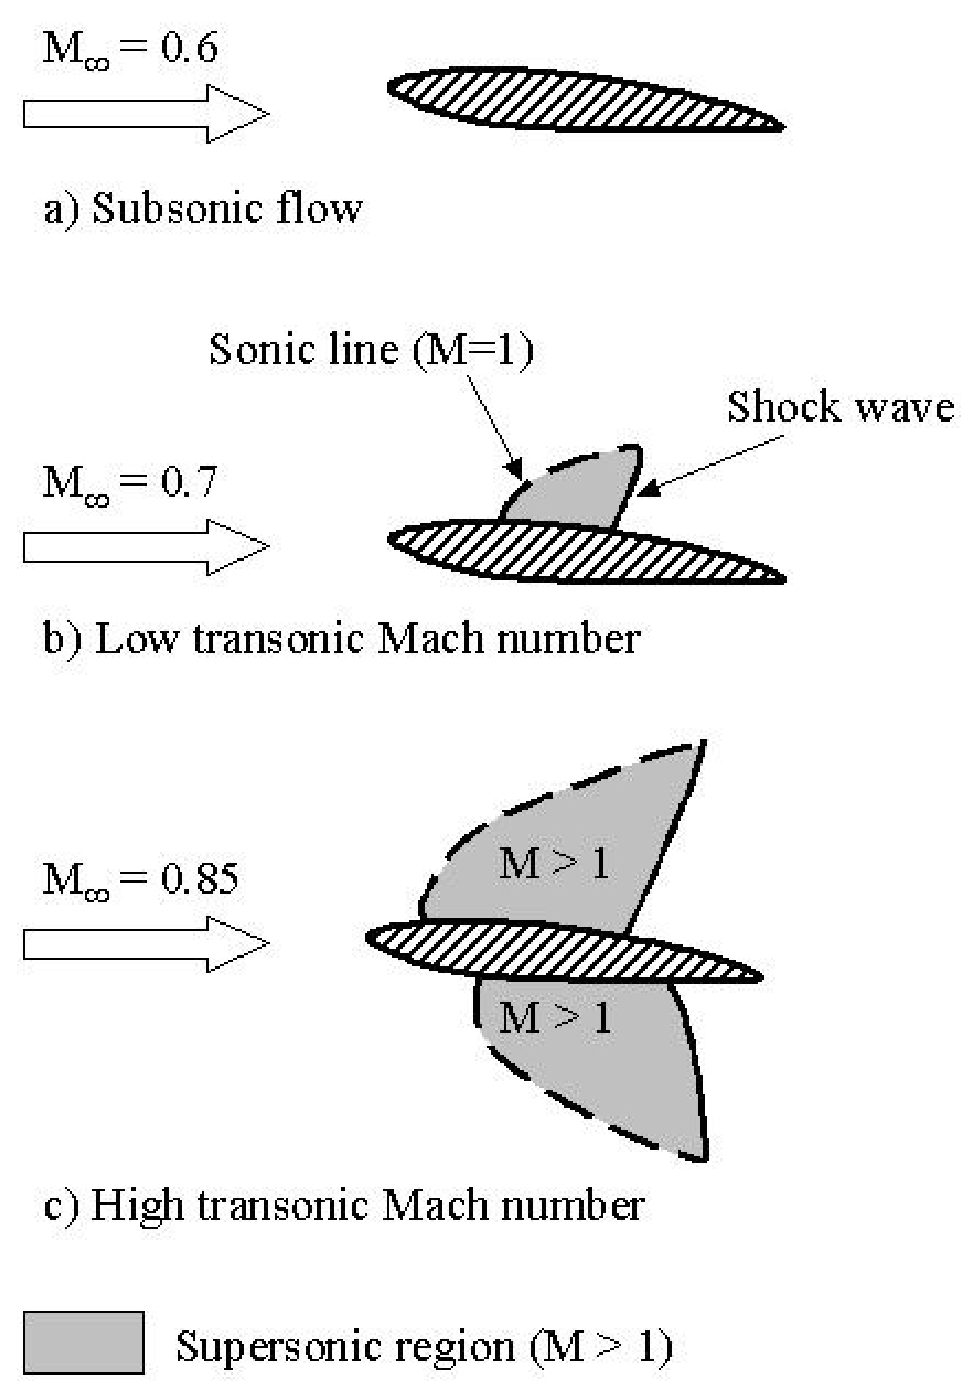
\includegraphics[bb = 92 86 545 742, height=6in]{aflow}
    \fi
    \caption{Airfoil Picture}
    \label{FigAir}
  \end{center}
\end{figure}

% above code has been macro-fied in Classes/MacroFile.tex file
%\InsertFig{\IncludeGraphicsH{aflow}{6in}{92 86 545 742}}{Airfoil Picture}{FigAir}

So as we have now labelled it we can reference it, like so (\ref{FigAir}) and it
is on Page \pageref{FigAir}. And as we can see, it is a very nice picture and we
can talk about it all we want and when we are tired we can move on to the next
chapter ...

Typewriter font: \texttt{This is from a typewriter}
Sans: \textsf{Sans serif yes yes}
Verbatim: \verb"Verbatim yes... code"
Roman: \textrm{Roman times perhaps?}

I would also like to add an extra bookmark in acroread like so ...
\ifpdf
test
  \pdfbookmark[2]{bookmark text is here}{And this is what I want bookmarked}
\fi
% ------------------------------------------------------------------------


%%% Local Variables:
%%% mode: latex
%%% TeX-master: "../thesis"
%%% End:

\chapter{Transient classification}
% Single source Bayesian template based classification
% % Mean template
% % % ML
% % % MAP
% % Multiple components
% Multi source Bayesian template based classification (multi mic or accelerometer)



\ifpdf
    \graphicspath{{Chapter2/Chapter2Figs/PNG/}{Chapter2/Chapter2Figs/PDF/}{Chapter2/Chapter2Figs/}}
\else
    \graphicspath{{Chapter2/Chapter2Figs/EPS/}{Chapter2/Chapter2Figs/}}
\fi

\section{First Section}
And now I begin my second chapter here ...

\section{Second Section}
and here I write more ...

\subsection{first subsection in the Second Section}
... and some more ...

\subsection{second subsection in the Second Section}
... and some more ...

\subsection{third subsection in the Second Section}
... and some more ...

% ------------------------------------------------------------------------

%%% Local Variables:
%%% mode: latex
%%% TeX-master: "../thesis"
%%% End:

\chapter{Restoration of transient noise}
% AR interpolation
% White noise substitution


\ifpdf
    \graphicspath{{Chapter3/Chapter3Figs/PNG/}{Chapter3/Chapter3Figs/PDF/}{Chapter3/Chapter3Figs/}}
\else
    \graphicspath{{Chapter3/Chapter3Figs/EPS/}{Chapter3/Chapter3Figs/}}
\fi

\section{First Section of the Third Chapter}
And now I begin my third chapter here ...

\subsection{first subsection in the First Section}
... and some more

\subsection{second subsection in the First Section}
... and some more ...

\subsubsection{first subsub section in the second subsection}
... and some more in the first subsub section otherwise it all looks the same
doesn't it? well we can add some text to it ...

\subsection{third subsection in the First Section}
... and some more ...

\subsubsection{first subsub section in the third subsection}
... and some more in the first subsub section otherwise it all looks the same
doesn't it? well we can add some text to it and some more and some more and
some more and some more and some more and some more and some more ...

\subsubsection{second subsub section in the third subsection}
... and some more in the first subsub section otherwise it all looks the same
doesn't it? well we can add some text to it ...

\section{Second Section of the Third Chapter}
and here I write more ...

% ------------------------------------------------------------------------


%%% Local Variables:
%%% mode: latex
%%% TeX-master: "../thesis"
%%% End:

0\def\baselinestretch{1}
\chapter{Conclusions}\label{ch:Conclusions}
\ifpdf
    \graphicspath{{Conclusions/ConclusionsFigs/PNG/}{Conclusions/ConclusionsFigs/PDF/}{Conclusions/ConclusionsFigs/}}
\else
    \graphicspath{{Conclusions/ConclusionsFigs/EPS/}{Conclusions/ConclusionsFigs/}}
\fi

\def\baselinestretch{1.66}

% Possible to accurately estimate the origin of touch interactions. Dependent on scenario... background noise... temperature shifts... sampling rate... device size... microphone placement and type.

This thesis has explored two aspects of impact induced pulses in real-time audio streams. Firstly a functional view of pulses that aimed to localise impact sites of touch events solely based on the resulting pulses in the audio stream for primarily single-channel applications with a multi-channel extension. This application was referred to as acoustic pulse recognition (APR) and at its core relied on being able to distinguish some minute variations in transient pulses while accepting other variations. Factors such as background noise, tapping style, strength and apparatus and even environmental temperature was shown to have a significant effect on the pulse waveform, an effect that the algorithm would have to be able to deal with. A range of waveform matching algorithms were developed, tested and some applications were tested and hypothesised.
Secondly, the pulses were considered noise and a real-time single-channel detection and restoration system was constructed for a telecommunication application. Various detection algorithms were proposed and tested, but for the unsupervised generally applicable case some key observations about the noise pulses were the guiding principles of work: noise pulses were typically broad-spectrum events with rapid changing energy levels which formed the necessary contrast to speech signals. After successful detection the restoration stage was considered from a two-level perspective based on the pre-processing stage used for the application. A set of largely clean tonal atoms and the residual. Here the residual was considered as the primary focus for the array of restoration approaches trialled, but heuristic approaches were explored for the restoration of noise polluted tonal components as well. 

This brief concluding chapter proceeds by summing up relevant results from throughout the thesis whereafter overall conclusions are presented based on the aims set out in the introduction. Finally selected suggestions for future work are presented.

\section{Summary of results}
Results presented in chapters~\ref{ch:APR} and~\ref{ch:MultichannelAPR} indicate a false classification rate of less, and in some cases far less, than 10 \% in the ideal environment. Both the single- and multi-channel systems were negatively affected by coloured background noise, but the multi-channel system managed to retain a near perfect classification rate. Extending the single-channel PCA model to include the amplitude, or scale, of the pulse as a random parameter increased performance while computational complexity scaled linearly with $L$ number of scales introduced. $L=20$ scales were found to be sufficient above which no performance increase was detected. The PCA factorisation approach achieved a high degree of separability between components and $I=3$ was found to be an adequate number of components in relation to the component number's influence on performance, and template lengths of about 120 samples equally seemed to indicate the point of diminishing returns for the system.

Results from the detection algorithm was presented in chapter~\ref{ch:TransientNoiseDetection} where two wavelet based detectors were presented both showing similar or better performance characteristics than comparable methods from the literature with the added advantage of higher temporal resolution. A pre-processing stage was presented that took advantage of the tonality of speech which was shown to effectively separate speech and transient noise both audibly and visibly. The pre-processing stage also provided the basis for the two-level approach to restoration proposed in chapter~\ref{ch:TransientNoiseRestoration} where the tonal and residual components were treated separately, if at all necessary in the case of the tonal components. A variety of objective perceptual methods showed general modest improvements of 0.2 MOS and 0.4 for PEAQ for the selected sets which in subjective tests were not favored by listeners. Overall subjective tests also revealed a slight preference to the restored samples with huge variability in preference between different sets tested.

\section{Evaluation of results}
Work presented on the functional aspects of impact induced audio pulses have clearly shown that it is possible to implement a simple touch based user interface system using APR with only one active channel. Allowing for more computationally intensive methods (K-PCA) increased performance significantly in clean as well as noisy environment. Even the simpler univariate methods outperformed the random chance baseline by a margin. The more advanced PCA based method proved more resilient to the common variability in pulse waveforms associated with a variety of factors if these could be incorporated into the model during training while the simpler methods failed in this regard. A multi-channel extension/generalisation of APR further increased classification performance to near perfect levels with the testing data used and in the testing scenarios. 

The concept of a single-channel APR system has been proposed and clearly shown to be a possible and feasible solution to the problem of touch interactive user interfaces. Some key difficulties have been explored and to a large part tackled, such as variability in tapping styles and strength. 
%possibly more here though?

A noise pulse detection and restoration system for the telecommunication application was designed and realised. Tests show that a real-time unsupervised single-channel keyboard typing suppression system is viable both subjectively and objectively. The detection system performs similarly or better than state of the art alternatives using more limited approaches. The proposed method requires a minimum of look-ahead time and provides a much higher temporal resolution than alternative methods due to the application of the wavelet basis. The separation stage and the two-level restoration enables a scalable restoration approach with tonal restoration providing an additional line of restoration for keyboard pulses showing strong tonal components. The high temporal resolution would in particular be of utility in scenarios with corruption of far shorter extent such as clicks or transmission errors.



\section{Suggestions for future research}

%http://www.devstud.org.uk/downloads/4be165997d2ae_Writing_the_Conclusion_Chapter,_the_Good,_the_Bad_and_the_Missing,_Joe_Assan%5B1%5D.pdf


%The conclusion chapter should have a definitive introduction which draws the attention of the
%reader to the thesis statement upon which the research was conducted. The introduction
%should restate the research question that the study set out to answer and clearly justify the
%necessity of such a course. There is also the need to establish the context, background
%and/or importance of the topic. Conversely, this section must indicate a problem, controversy
%or a gap in the field of study. In doing this it is proper that the research questions are outlined
%and the key objectives of the study.
%
%Secondly, the introduction of the conclusion, just like those of the discussion chapters should
%provide a map of how the chapter has been structured. It should therefore provide a pictorial
%sequence of the issues to be discussed and how the section will end. This allows the
%examiner the opportunity to know what to expect and strong grounding for the research
%coverage.


%%% ----------------------------------------------------------------------

% ------------------------------------------------------------------------

%%% Local Variables:
%%% mode: latex
%%% TeX-master: "../thesis"
%%% End:


\appendix
\chapter{Appdx A}

and here I put a bit of postamble ...

% ------------------------------------------------------------------------

%%% Local Variables: 
%%% mode: latex
%%% TeX-master: "../thesis"
%%% End: 

\chapter{Appdx B}

and here I put some more postamble ...

% ------------------------------------------------------------------------

%%% Local Variables: 
%%% mode: latex
%%% TeX-master: "../thesis"
%%% End: 




%\bibliographystyle{Classes/CUEDbiblio}
%\bibliographystyle{Classes/jmb}
%\bibliographystyle{plainnat} %this works with package natbib
\bibliographystyle{Classes/jmb} % bibliography style
\renewcommand{\bibname}{References} % changes default name Bibliography to References
\bibliography{References/references} % References file
\addcontentsline{toc}{chapter}{References} %adds References to contents page


\end{document}
